
\let\negmedspace\undefined
\let\negthickspace\undefined
\documentclass[journal]{IEEEtran}
\usepackage[a5paper, margin=10mm, onecolumn]{geometry}
%\usepackage{lmodern} % Ensure lmodern is loaded for pdflatex
\usepackage{tfrupee} % Include tfrupee package

\setlength{\headheight}{1cm} % Set the height of the header box
\setlength{\headsep}{0mm}     % Set the distance between the header box and the top of the text

\usepackage{gvv-book}
\usepackage{gvv}
\usepackage{cite}
\usepackage{amsmath,amssymb,amsfonts,amsthm}
\usepackage{algorithmic}
\usepackage{graphicx}
\usepackage{textcomp}
\usepackage{xcolor}
\usepackage{txfonts}
\usepackage{listings}
\usepackage{enumitem}
\usepackage{mathtools}
\usepackage{gensymb}
\usepackage{comment}
\usepackage[breaklinks=true]{hyperref}
\usepackage{tkz-euclide} 
\usepackage{listings}
% \usepackage{gvv}                                        
\def\inputGnumericTable{}                                 
\usepackage[latin1]{inputenc}                                
\usepackage{color}                                            
\usepackage{array}                                            
\usepackage{longtable}                                       
\usepackage{calc}                                             
\usepackage{multirow}                                         
\usepackage{hhline}                                           
\usepackage{ifthen}                                           
\usepackage{lscape}
\begin{document}

\bibliographystyle{IEEEtran}
\vspace{3cm}

\title{1.1.5.6}
\author{AI24BTECH11005 - Bhukya Prajwal Naik
}
% \maketitle
% \newpage
% \bigskip
{\let\newpage\relax\maketitle}

\renewcommand{\thefigure}{\theenumi}
\renewcommand{\thetable}{\theenumi}
\setlength{\intextsep}{10pt} % Space between text and floats


\numberwithin{equation}{enumi}
\numberwithin{figure}{enumi}
\renewcommand{\thetable}{\theenumi}


\textbf{Question}:\\
 The point which divides the line segment joining the points \myvec{7 \\ -6} ,\myvec{3 \\ 4} in the ratio 1:2 is .
\solution

\begin{table}[h!]
	\centering
	\begin{tabular}[12pt]{|c|c|c|}
    \hline
	\textbf{Information} & \textbf{Symbolic form} & \textbf{Value}\\ 
    \hline
	Given Line & $\vec{X} = \vec{h}+k\vec{m}$ & $x+y=6$\\
    \hline 
	Direction vector & $\vec{m}$ & \myvec{1 \\ -1}\\
    \hline
	Normal vector & $\vec{n}$ & \myvec{1 \\ 1}\\
    \hline   
    \end{tabular}

	\caption{Coordinates of points involved}
	\label{tab:coordinates}
\end{table}

Given, P divides the line segment AB in ratio 1:2.

Using the section formula,

\begin{align}
	\vec{P} &= \frac{1}{1+k}\myvec{\vec{A} & \vec{B}}\myvec{1 \\ k} \\[5pt]
	\vec{P} &= \frac{1}{1+\frac{1}{2}}\myvec{7 &3\\-6 & 4}\myvec{1 \\ \frac{1}{2}}\\[5pt]
	\vec{P} &= \myvec{\frac{17}{3} \\ \frac{-8}{3}}
\end{align}

\begin{figure}[h!]
	\centering
	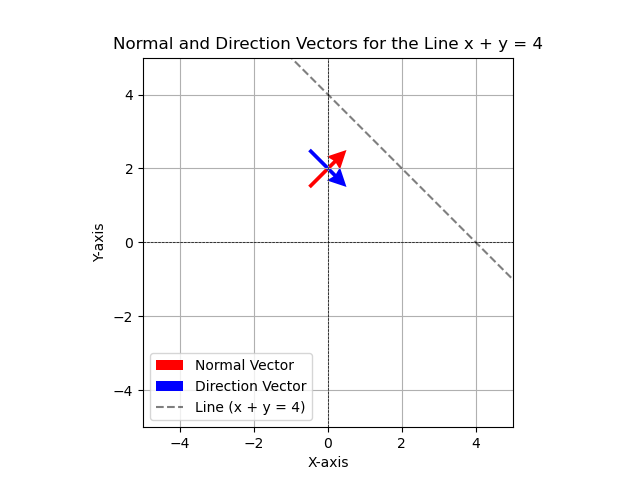
\includegraphics[width=0.7\textwidth]{Figure_1.png}
	\label{Graph}
	\caption{Plot of points A,B,P}
        \end{figure}




\end{document}
